\documentclass{article}

\usepackage{xcolor}
\usepackage{microtype}
\usepackage{graphicx}
\usepackage{subfigure}
\usepackage{booktabs}
\usepackage{multirow}
\usepackage{array}
\usepackage{amsmath}
\usepackage{amssymb}
\usepackage{hyperref}
\usepackage[normalem]{ulem}

\newcommand{\theHalgorithm}{\arabic{algorithm}}

\usepackage{mlsys2025}
\hypersetup{hypertexnames=false}

\usepackage{xspace}
\usepackage{enumitem}
\usepackage{pgfplots}
\usepackage{adjustbox}
\usepackage{placeins}
\pgfplotsset{compat=1.17}
\usetikzlibrary{arrows.meta,positioning,calc}
\definecolor{cLin}{HTML}{2A78D6}
\definecolor{cHeavy}{HTML}{EB6834}
\definecolor{cInk}{HTML}{52514E}
\definecolor{cMuted}{HTML}{898781}
\definecolor{cGrid}{HTML}{E1E0D9}
\definecolor{cAxis}{HTML}{C3C2B7}
\definecolor{cObsFill}{HTML}{EEF4FC}
\definecolor{cGood}{HTML}{3C9D5D}
\definecolor{cGoodFill}{HTML}{E5F3E9}
\definecolor{cBad}{HTML}{D2504B}
\definecolor{cBadFill}{HTML}{FBE7E6}
\definecolor{cNeg}{HTML}{E34948}
\pgfplotsset{
  paperplot/.style={
    font=\scriptsize, tick label style={font=\scriptsize}, label style={font=\scriptsize},
    axis line style={cAxis}, tick style={cAxis}, major grid style={cGrid, thin},
    every axis legend/.append style={draw=none, fill=none, font=\scriptsize},
    legend cell align=left, /tikz/every mark/.append style={solid}},
  diverging/.style={colormap={div}{rgb255=(42,120,214) rgb255=(240,239,236) rgb255=(227,73,72)}},
}
\newcommand{\figdata}{figures/data}
\newcommand{\xv}{xv6-riscv\xspace}
\newcommand{\clock}{Clock\xspace}
\newcommand{\belady}{Belady\xspace}

\newcommand{\tierF}{\textsf{F}\xspace}
\newcommand{\tierK}{\textsf{K}\xspace}
\newcommand{\tierKp}{\textsf{K+}\xspace}
\newcommand{\tierKKp}{\textsf{K}$\cup$\textsf{K+}\xspace}
\newcommand{\feat}[1]{\texttt{#1}}

\newcommand{\wsixteen}{figures/data/w16}
\newcommand{\wfifteen}{../week_15_update/tables}
\newcommand{\best}[1]{\textbf{#1}}

\newcommand{\todo}[1]{\textcolor{red}{[TODO: #1]}}
\newcommand{\plan}[1]{\textcolor{blue!60!black}{\textit{[Plan: #1]}}}
\newcommand{\verify}[1]{\textcolor{orange!80!black}{[verify: #1]}}

\newcommand{\figbox}[3]{%
  \fbox{\parbox[c][#1][c]{0.94\linewidth}{\centering\small
    \textbf{Planned figure.} #2\\[3pt]
    \textcolor{blue!60!black}{\footnotesize Source/status: #3}}}}
\newcommand{\figboxwide}[3]{%
  \fbox{\parbox[c][#1][c]{0.96\textwidth}{\centering\small
    \textbf{Planned figure.} #2\\[3pt]
    \textcolor{blue!60!black}{\footnotesize Source/status: #3}}}}

\newcommand{\finding}[1]{\textbf{#1}\hspace{0.4em}}
\newcommand{\obs}[2]{\textbf{Observation #1: #2}\hspace{0.4em}}
\newcommand{\rqbox}[3]{\par\smallskip\noindent\textbf{#1.} \emph{#2} #3\par}

\newif\ifwithappendix
\withappendixtrue

\graphicspath{{figures/}{../figures2/}}

\mlsystitlerunning{Lightweight ML-Guided Page Replacement}

\begin{document}

\twocolumn[
\mlsystitle{Can Lightweight ML-Guided Page Replacement Manage Memory Better Than Classical Policies?}

\begin{mlsysauthorlist}
\mlsysauthor{Anonymous Author 1}{anon}
\mlsysauthor{Anonymous Author 2}{anon}
\end{mlsysauthorlist}
\mlsysaffiliation{anon}{Anonymous Institution} \mlsyscorrespondingauthor{Anonymous Author 1}{anonymous@anonymous.invalid}

\mlsyskeywords{Machine Learning for Systems, Operating Systems, Page Replacement, Learned Policies}

\vskip 0.3in

\begin{abstract}
Learned policies have improved caching in CPUs and content-delivery networks, but they are hard to use for page replacement inside an operating-system kernel: the kernel cannot see individual memory accesses, cannot use floating point when it evicts a page, and every eviction changes later faults. We build PageScore, a learned page-replacement policy for the xv6 kernel. It scores 32 randomly chosen pages with a small integer model over information the kernel already keeps, such as whether a page was recently used, written to, or evicted and needed again, and it is trained offline to copy \belady's optimal policy. Across 14 workloads, eight of them never used in training, it causes 8.8\% fewer page faults than \clock at 10\% memory and 9.8\% fewer at 20\%. It does not beat the best classical policies, ARC and LHD, but matches them at a lower cost per decision except on the smallest memories, a cost that barely grows with memory. Larger learned models do no better, and with the disks and processor we measured, the faults PageScore saves pay for the time it spends choosing.
\end{abstract}
]

\printAffiliationsAndNotice{}

\section{Introduction}
\label{sec:intro}

\begin{table}[t]
\caption{\textbf{Measured in the xv6 kernel:} page faults relative to \clock (lower is better) when each program may keep 5, 10 or 20\% of its pages, averaged over 14 workloads, and the instructions needed to choose one page to evict among 68 and 516 pages. Bold: the whole 95\% interval is below 0.99 (\S\ref{sec:eval-setup}). $^\dagger$Using only the accessed bit (\S\ref{sec:impl}). PageScore, our policy, beats \clock at 10\% and 20\%, is level with ARC, and its cost barely grows with memory.}
\label{tab:teaser}
\vskip 0.1in
\begin{center}
\begin{small}
\setlength{\tabcolsep}{2.5pt}
\begin{tabular}{@{}lrrrrr@{}}
\toprule
 & \multicolumn{3}{c}{faults / \clock} & \multicolumn{2}{c}{instr./eviction} \\
\cmidrule(lr){2-4}\cmidrule(l){5-6}
Policy & 5\% & 10\% & 20\% & 68 & 516 \\
\midrule
FIFO                 & 1.228 & 1.253 & 1.345 & 384    & 2,624 \\
Aging                & 1.043 & 1.066 & 1.166 & 8,124  & 60,978 \\
LFU                  & 1.068 & 1.130 & 1.270 & 8,004  & 59,980 \\
\clock               & 1.000 & 1.000 & 1.000 & 410    & 1,068 \\
LeCaR$^\dagger$      & 1.051 & 1.113 & 1.212 & 8,156  & 60,678 \\
S3-FIFO$^\dagger$    & 1.086 & 1.016 & 1.086 & 1,395  & 6,452 \\
LHD$^\dagger$        & 1.005 & 0.951 & 0.949 & 14,397 & 111,705 \\
ARC$^\dagger$        & \textbf{0.947} & \textbf{0.943} & 0.984 & 11,934 & 81,070 \\
\midrule
PageScore (ours) & 0.972 & \textbf{0.912} & \textbf{0.902} & 8,480 & 8,895 \\
\quad every page & 0.976 & \textbf{0.914} & 0.882 & 16,818 & 134,392 \\
\bottomrule
\end{tabular}
\end{small}
\end{center}
\vskip -0.1in
\end{table}

When a program needs more memory than it is allowed, some of its pages must be moved out to disk, and every access to a swapped-out page becomes a page fault: a slow read from the device. Reading one page takes about 63\,\textmu s on our SSD and 8.9\,ms on our hard disk (Appendix, Table~\ref{tab:breakeven}). The eviction policy determines which pages to remove, directly impacting how many page faults occur.

The kernel must choose without knowing which pages the program will need next. It relies on the hardware's accessed bit, which marks the pages a program has used since the kernel last checked (\S\ref{sec:bg-mechanism}), and on simple rules built on it, such as \clock and its successors~\citep{corbato1968paging,carr1981wsclock} and, in Linux, the multi-generational LRU~\citep{linux_mglru}. These rules leave many faults that could be avoided: on several of our workloads, \belady's optimal policy~\citep{belady1966study}, which knows the future, causes about half as many faults as \clock (\S\ref{sec:bg-headroom}). Stronger policies such as ARC~\citep{megiddo2003arc}, LHD~\citep{beckmann2018lhd} and S3-FIFO~\citep{yang2023s3fifo} were designed for caches that see every access. When adapted to use only the accessed bit, top cache policies like ARC reduce faults by just around 5\% relative to \clock at small memory limits (Table~\ref{tab:teaser}).

Learned policies already beat hand-written ones in CPU caches and in web and storage caches~\citep{jain2016hawkeye,vietri2018lecar,shi2019glider,song2020lrb,rodriguez2021cacheus,shah2022mockingjay,song2023halp}, but there they see every access, and they run outside the kernel in floating point. A kernel sees far less: it only learns about a page when the page faults, when a page it evicted is needed again (a \emph{refault}), or when a check finds that the page was used or written, and it must choose a page quickly, without floating point. Learning in memory management has so far placed pages across memory tiers or tuned settings~\citep{doudali2019kleio,lagarcavilla2019farmemory,ramaswamy2026xtier}, and the closest eviction work, LearnedCache~\citep{qi2026learnedcache}, handles file pages rather than a program's own memory (\S\ref{sec:related}). We found no learned policy that evicts a program's own memory using only what a kernel sees.

We ask whether a learned page-replacement policy can work at operating-system level with only the signals a kernel observes, without floating point, on the eviction path, and without knowing which program it serves. Our answer is a qualified yes: \textbf{the kernel already sees enough}. Our policy, \textit{PageScore}, is a small linear score over information the kernel already keeps, computed in whole numbers for $n$ randomly chosen pages. For our case, where we used $n = 32$, it causes 8.8\% fewer page faults than \clock at 10\% memory and 9.8\% fewer at 20\%, and matches ARC and LHD, the best classical policies a kernel can run, at a lower cost per decision except on the smallest memories. Counting disk reads, writes and decision time at 10\% memory, it takes 8--9\% less time than \clock on both our hard disk and our SSD with our desktop processor. 

Five design choices make this work inside a kernel. The score uses the accessed and dirty bits and refault counts, because the kernel never sees individual accesses (\S\ref{sec:design-features}). Training always includes the most recently used pages, and new pages are protected for a short time, because otherwise the policy learns to evict the page that is in use (\S\ref{sec:design-train}). The score uses only integers (\S\ref{sec:design-int}). Features and probation are chosen on validation streams, never on test streams, and the kernel checks every page the model picks (\S\ref{sec:design-wrong}). Scoring only 32 pages keeps each decision cheap however much memory a program has (\S\ref{sec:design-cost}). 

Our contributions are:
\begin{itemize}[topsep=3pt, itemsep=2pt, parsep=0pt]
\item \textbf{A learned page-replacement policy that runs inside a kernel at the cost of a classical one}: an integer score over 32 sampled pages, and five larger models that also run in the kernel using only integers (\S\ref{sec:design}, \S\ref{sec:impl}).
\item \textbf{A study of what a learned eviction policy needs.} Extra information that a kernel does not have helps only on the programs a model was trained on, and larger models do not help (\S\ref{sec:bg}, \S\ref{sec:eval-info}, \S\ref{sec:eval-ablate}).
\item \textbf{An evaluation inside the kernel}: 14 workloads, three memory sizes and 4,489 kernel runs, against \clock, ARC, LHD, S3-FIFO and LeCaR, with exact decision costs and measured disk speeds (\S\ref{sec:eval}).
\item \textbf{A paging platform and dataset for xv6}: demand paging and swap, and complete traces of every read and write, checked against independent models of each program (\S\ref{sec:impl}, Appendix~\ref{app:data}).
\end{itemize}

\section{Background and Motivation}
\label{sec:bg}

\subsection{Page Replacement, as the Kernel Sees It}
\label{sec:bg-mechanism}

Each program may keep only a limited number of pages in memory. When it touches a page that is not in memory, the hardware traps into the kernel: a page fault. If the program is at its limit, the kernel picks one of the program's own pages to evict (the \emph{victim}), writes it to swap if it has changed, and loads the needed page in its place (Figure~\ref{fig:mechanism}). This choice is made once per eviction while the program waits, so its cost adds to the fault. The kernel never sees the program's individual memory accesses: the hardware only sets a page's accessed bit when the page is used and its dirty bit when it is written, and the kernel reads and clears these bits when it scans the pages at an eviction. \clock uses the accessed bit to give recently used pages a second chance, and Aging keeps a short history of it for each page. \belady's policy, which evicts the page whose next use is furthest in the future, is the best possible policy for faults, though not for writes. Linux can limit a program's memory in the same way.

\begin{figure}[t]
\centering
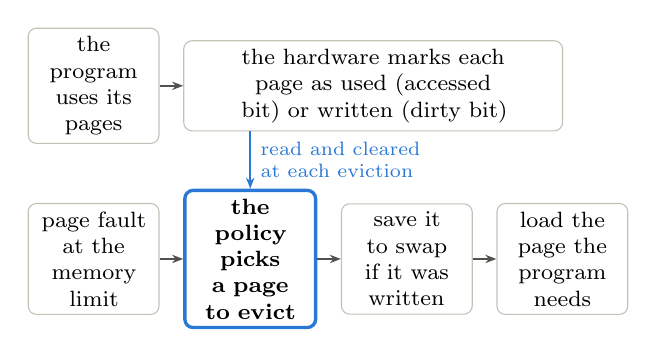
\begin{tikzpicture}[font=\footnotesize, node distance=0.3cm,
  box/.style={draw=cAxis, rounded corners=3pt, align=center, inner sep=3pt, minimum height=1.05cm, text width=1.45cm},
  key/.style={box, draw=cLin, very thick},
  flow/.style={-{Stealth[length=4pt]}, cInk, thick}]
\node[box] (fault) {page fault at the memory limit};
\node[key, right=of fault] (pick) {\textbf{the policy picks a page to evict}};
\node[box, right=of pick] (save) {save it to swap if it was written};
\node[box, right=of save] (load) {load the page the program needs};
\node[box, above=0.75cm of fault] (prog) {the program uses its pages};
\node[box, right=of prog, text width=4.6cm] (bits) {the hardware marks each page as used (accessed bit) or written (dirty bit)};
\draw[flow] (fault) -- (pick); \draw[flow] (pick) -- (save); \draw[flow] (save) -- (load);
\draw[flow] (prog) -- (bits);
\draw[flow, cLin] (pick |- bits.south) -- node[right, font=\scriptsize, text=cLin, align=left] {read and cleared\\at each eviction} (pick.north);
\end{tikzpicture}
\caption{The eviction path. The policy decides once per eviction, while the program waits, and sees only the accessed and dirty bits, never the program's individual memory accesses.}
\label{fig:mechanism}
\end{figure}

\subsection{Simple Rules Are Far from Optimal}
\label{sec:bg-headroom}

\finding{Workloads.} We use fourteen workloads, each run on several inputs that we call streams (Table~\ref{tab:workloads}). The models are trained on six: a B+-tree (btree), BFS and PageRank on a graph (graph), a hash table (kv), LZW compression (lzw), matrix multiply (matmul) and merge sort (sort). The other eight were never used to train or choose a model: the hash table replaying real Twitter cache traces~\citep{yang2020twitter} taken from \citet{zussman2025cacheext} (kv-T), heap allocation churn (heap), a hash join (join), sparse matrix--vector product (spmv), pointer chasing (chase), Bloom-filter lookups (bloom), simple synthetic access patterns (pat) and four programs that imitate real applications (app). Not all of these are new programs: kv-T runs the trained hash table on real traffic. Each workload's streams are split into training, validation and test streams, and some whole variants are kept for testing only (held out); Appendix~\ref{app:data} gives the details.

\begin{table}[t]
\caption{Workloads. The learned models are trained on the six marked ``train'' and run
unchanged on the other eight.}
\label{tab:workloads}
\vskip 0.05in
\begin{center}
\begin{footnotesize}
\setlength{\tabcolsep}{3pt}
\begin{tabular}{@{}l>{\raggedright\arraybackslash}p{1.95in}l@{}}
\toprule
Workload & What it is & Training \\
\midrule
btree  & B+-tree, 4\,KB nodes (SQLite-pager-like)                & train \\
graph  & BFS and PageRank, scale-free graph                       & train \\
kv     & Zipfian hash table, YCSB mixes (Redis-like)              & train \\
lzw    & LZW compression (\texttt{compress(1)})                   & train \\
matmul & naive vs.\ blocked matrix multiply                       & train \\
sort   & bottom-up merge sort                                     & train \\
\midrule
kv-T   & kv replaying Twitter cache traces                        & -- \\
heap   & \texttt{malloc}/\texttt{free} churn                      & -- \\
join   & hash join, build and probe                               & -- \\
spmv   & sparse matrix--vector product (CSR)                      & -- \\
chase  & serial pointer chasing                                   & -- \\
bloom  & Bloom-filter probes                                      & -- \\
pat    & 11 synthetic patterns (loop, Zipf, phase, \ldots)        & -- \\
app    & four application-shaped programs                         & -- \\
\bottomrule
\end{tabular}
\end{footnotesize}
\end{center}
\end{table}

\obs{1}{\clock is close to exact LRU, and both are far from optimal.} On the six training workloads, \clock comes within 2\% of exact LRU, which evicts the least recently used page, on five of them. Exact LFU, which evicts the least often used page, helps on btree but fails badly on graph, sort and matmul. \belady's policy causes 17--54\% fewer faults than \clock on these workloads (Figure~\ref{fig:headroom}). \emph{How recently and how often a page was used both help, but every fixed way of combining them fails on some workload; a policy should learn the combination}.

\begin{figure}[t]
\centering
\begin{tikzpicture}
\begin{axis}[paperplot, width=\linewidth, height=1.42in, tick pos=left,
  xmin=0.25, xmax=1.56, ymin=-0.6, ymax=5.6, y dir=reverse,
  ytick={0,...,5}, yticklabels={btree,graph,kv,lzw,matmul,sort},
  xtick={0.4,0.6,0.8,1.0,1.2,1.4}, xmajorgrids,
  xlabel={faults relative to \clock}, xlabel style={yshift=3pt},
  legend style={at={(0.5,1.02)}, anchor=south, legend columns=-1,
    /tikz/every even column/.append style={column sep=6pt}}]
\addplot[cInk, thin, forget plot] coordinates {(1,-0.6) (1,5.6)};
\addplot[only marks, mark=*, mark size=1.5pt, cInk, fill opacity=0.75, draw opacity=0.75]
  table[x=ratio, y=row, col sep=comma] {\figdata/headroom_classical.csv};
\addlegendentry{FIFO, Aging, LFU, LRU, exact LFU}
\addplot[only marks, mark=triangle*, mark size=2pt, mark options={rotate=-90}, cInk,
  forget plot] table[x=ratio, y=row, col sep=comma] {\figdata/headroom_clipped.csv};
\addplot[only marks, mark=*, mark size=2.2pt, cLin,
  error bars/.cd, x dir=plus, x explicit, error mark=none,
  error bar style={cLin, line width=1.2pt}]
  table[x=ratio, y=row, x error=gap, col sep=comma] {\figdata/headroom_belady.csv};
\addlegendentry{\belady}
\addplot[only marks, mark=none, nodes near coords, point meta=explicit symbolic,
  every node near coord/.append style={anchor=east, font=\tiny, text=cLin, xshift=-2pt},
  forget plot]
  table[x=ratio, y=row, meta=label, col sep=comma] {\figdata/headroom_belady.csv};
\end{axis}
\end{tikzpicture}
\caption{How far each policy is from \belady (simulator, averaged over 5, 10 and 20\% memory; test streams, and held-out streams for matmul). The blue line is the gap between \belady and the best grey dot. Values beyond the axis (exact LFU on graph, sort and matmul, about 3$\times$ \clock's faults) are drawn at the edge.}
\label{fig:headroom}
\end{figure}

\subsection{What a Learned Policy Needs}
\label{sec:bg-signals}\label{sec:bg-naive}

\obs{2}{What the kernel can see is nearly as useful as a full trace.} For each eviction, we check how well each piece of information orders the pages by when they will next be used (Appendix, Figure~\ref{fig:diagnostics}). The kernel's rough access count, built from the accessed bits it finds when it scans (\feat{sfreq}), does this about as well as the exact count that only a full trace gives (\feat{freq}), and the refault distance that Linux already records (\feat{rdist}) does better than both. \emph{The key could be to use information the kernel already has, and train and judge models on whole eviction decisions, not on single accesses} (\S\ref{sec:design-features}).

\obs{3}{A policy trained on randomly chosen pages evicts the page the program is using.} If each recorded eviction contains \belady's choice plus 31 randomly chosen pages, two thirds of the linear models trained on graph cause at least three times \clock's faults on a PageRank stream. A failing model evicts the page it has just loaded, which is needed again almost at once: among 167 pages in memory, the one or two just used are rarely in a random sample, so the model never learns to keep them. Retraining on the model's own decisions (DAgger~\citep{ross2011dagger}) rescues one model but not most of them (Appendix, Table~\ref{tab:dagger}). \emph{So training data must include recently used pages, and new pages need protection} (\S\ref{sec:design-train}).

\label{sec:bg-rq}Whether a learned policy can work in a kernel comes down to four questions, answered in \S\ref{sec:eval}:
\begin{description}[topsep=2pt, itemsep=1pt, parsep=0pt]
\item[RQ1 Information.] Is what the kernel already knows enough, or does a learned policy need information only a full trace has? (\S\ref{sec:eval-info})
\item[RQ2 Effect in the kernel.] Inside a real kernel, does the policy beat \clock and the best classical policies a kernel can run? (\S\ref{sec:eval-kernel})
\item[RQ3 Cost.] Can it run without floating point, what does each decision cost, and when do the faults it saves pay for it? (\S\ref{sec:eval-cost})
\item[RQ4 Robustness.] Does it work on programs it never saw, and where does it fail? (\S\ref{sec:eval-robust})
\end{description}

\section{Learning From What the Kernel Already Sees}
\label{sec:design}

\subsection{Overview}
\label{sec:design-overview}

PageScore is trained offline. We replay each training stream with LRU at 5, 10 and 20\% memory sizes, and at some of the evictions we record the pages in memory with their features and the right answer (\S\ref{sec:design-train}). We fit a linear model, choose on validation streams which features to use and for how many scans (0, 1, 2 or 4) a newly loaded page is protected from eviction, and round the weights to integers (Figure~\ref{fig:overview}).

In the kernel, at each eviction PageScore picks 32 of the program's pages in memory at random (all of them if there are fewer), updates their accessed-bit history, scores each with integer arithmetic, skips newly loaded pages, and evicts the page with the highest score (Algorithm~\ref{alg:choose}).

PageScore learns to copy \belady. For each page it predicts how far away the page's next use is, on a log scale, and evicts the page it expects to be needed last; the model is fitted in one step with ridge regression. Copying \belady works because our complete traces give the right answer for every decision offline, whereas reinforcement learning would have to experiment inside a running kernel. Because each eviction changes what happens later, we judge every policy by replaying whole streams, not by how often single predictions are right. One model, trained on all six training workloads, is used unchanged on every workload. We use a linear model because larger ones are no better for their cost (\S\ref{sec:eval-ablate}).

\begin{figure*}[t]
\centering
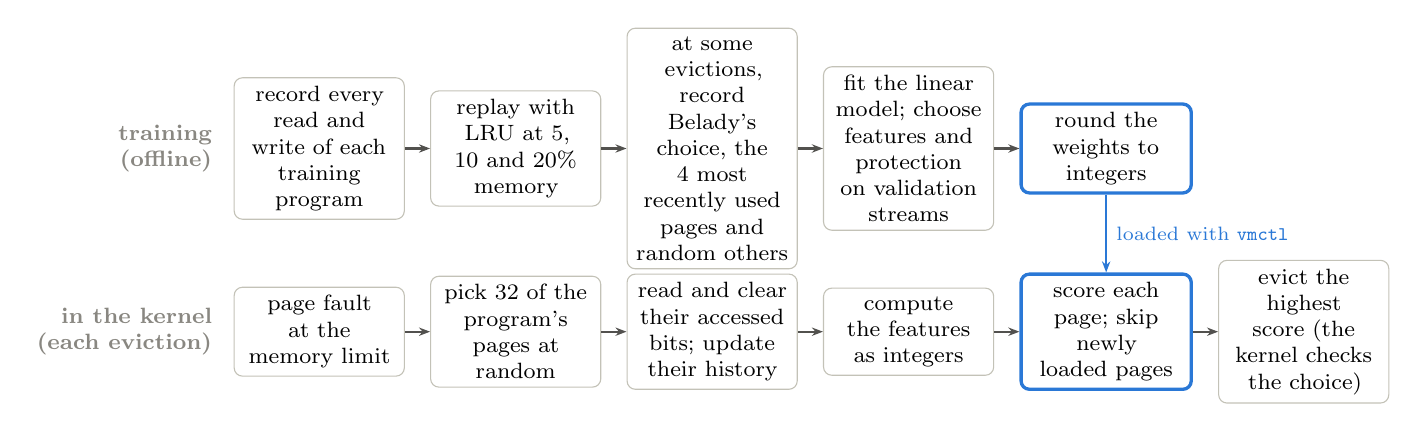
\begin{tikzpicture}[font=\footnotesize, node distance=0.32cm,
  box/.style={draw=cAxis, rounded corners=3pt, align=center, inner sep=3pt, minimum height=1.05cm, text width=1.95cm},
  key/.style={box, draw=cLin, very thick},
  flow/.style={-{Stealth[length=4pt]}, cInk, thick},
  lane/.style={font=\footnotesize\bfseries, text=cMuted, anchor=east, align=right}]
\node[box] (o1) {record every read and write of each training program};
\node[box, right=of o1] (o2) {replay with LRU at 5, 10 and 20\% memory};
\node[box, right=of o2] (o3) {at some evictions, record \belady's choice, the 4 most recently used pages and random others};
\node[box, right=of o3] (o4) {fit the linear model; choose features and protection on validation streams};
\node[key, right=of o4] (o5) {round the weights to integers};
\node[box, below=0.85cm of o1] (k1) {page fault at the memory limit};
\node[box, right=of k1] (k2) {pick 32 of the program's pages at random};
\node[box, right=of k2] (k3) {read and clear their accessed bits; update their history};
\node[box, right=of k3] (k4) {compute the features as integers};
\node[key, right=of k4] (k5) {score each page; skip newly loaded pages};
\node[box, right=of k5] (k6) {evict the highest score (the kernel checks the choice)};
\foreach \a/\b in {o1/o2,o2/o3,o3/o4,o4/o5,k1/k2,k2/k3,k3/k4,k4/k5,k5/k6}
  \draw[flow] (\a) -- (\b);
\draw[flow, cLin] (o5) -- node[right, font=\scriptsize, text=cLin] {loaded with \texttt{vmctl}} (k5);
\node[lane, left=0.15cm of o1] {training\\(offline)};
\node[lane, left=0.15cm of k1] {in the kernel\\(each eviction)};
\end{tikzpicture}
\caption{Overview of PageScore. Training happens offline and uses the future; in the kernel, PageScore adds only a scan the kernel already does and a few integer multiply-adds per sampled page.}
\label{fig:overview}
\end{figure*}

\subsection{Features and Training Data}
\label{sec:design-features}\label{sec:design-train}

A kernel never sees individual accesses (\S\ref{sec:bg-mechanism}), so PageScore uses only information a kernel can collect when it scans its pages at an eviction (group \tierK), plus the refault records that Linux already keeps (group \tierKp) (Appendix, Table~\ref{tab:features}). Time is counted in scans, one per eviction. A third group, \tierF, holds exact information only a full trace has, such as when each page was last used; we use it only to measure what extra information would be worth.

We train on recorded eviction decisions, and each one always includes the 4 most recently used pages, because a random sample of the pages in memory almost never contains the page just used (\S\ref{sec:bg-naive}). \emph{Probation} is added: a page loaded fewer than a set number of scans ago is not evicted while an older page is available, like \clock's second chance; the number of scans is chosen on validation streams. The training data has 5.2 million rows from 377,000 decisions.

\subsection{Running in the Kernel}
\label{sec:design-int}\label{sec:design-wrong}\label{sec:design-cost}

\finding{Integers only.} xv6 does not save floating-point registers when it switches between programs, and Linux does not normally allow floating point in kernel code~\citep{linux_fpu}, so PageScore computes only with integers. The score of a page is
\begin{equation}
s(\text{page}) = \sum_{j\in S} q_j\, X_j(\text{page}), \qquad
q_j = \operatorname{round}\!\left(\frac{w_j}{\sigma_j}\, 2^{b}\right),
\label{eq:score}
\end{equation}
where $X_j$ is feature $j$ stored as an integer with $b=8$ fractional bits, $S$ is the chosen set of features, $w_j$ is the learned weight and $\sigma_j$ the feature's spread, so each $q_j$ is an integer. The page with the highest score is the one the model expects to be needed last. The kernel and the simulator compute features with the same code, so a model scores a page the same way in both. PageScore's model uses five features and protects new pages for 4 scans. It evicts a page sooner the longer the page has sat idle, the farther apart its past refaults were, and if it was written to, and keeps pages that came back after an earlier eviction or have stayed in memory a long time.

\finding{Larger models.} To test whether a larger model helps, we also converted five larger models (a CNN over the aging bits, a deeper MLP, set-attention, boosted trees and ranking trees) to integer arithmetic; they run in both the kernel and the simulator.

\finding{When the model is wrong.} The worst possible case is that the policy causes more faults than \clock, not corruption: the policy can never evict another process's pages. The model can only pick the program's own pages to be evicted and the kernel checks every page it picks and falls back to \clock if the choice is not allowed. \emph{Probation} keeps new pages from being evicted, which removes the failure of \S\ref{sec:bg-naive}. Features and probation are chosen on validation streams, never on the test streams, because many feature sets fail badly. At 10\% memory, more than a third of them cause at least three times \clock's faults on graph. Nothing switches PageScore off while it runs, so it can still be worse than \clock on some workloads (\S\ref{sec:eval-loss}).
\finding{A fixed sample.} Scoring takes about the same work for every page, so scoring all of them gets slower as memory grows. PageScore therefore scores only $n$ randomly chosen pages, or all of them if there are fewer; in our implementation in xv6, $n=32$. A fixed $n$ is enough because how good a random sample is depends on its size, not on how many pages it is drawn from: the best page in a random sample of 32 is, on average, among the top 3\% of pages to evict, however many pages the program has (\S\ref{sec:discussion} discusses much larger memories). Table~\ref{tab:samples} shows the trade-off: fewer pages cost fewer instructions but cause more faults, while more than 32 pages cost more and save almost nothing, so 32 is where the curve flattens. We first picked 32 by trying several sample sizes on the test streams; a rule fixed in advance and applied only to the validation streams, the smallest sample within 1\% of scoring every page at all three memory sizes, also picks 32 (Figure~\ref{fig:dist}, right).

\begin{table}[t]
\caption{What each sample size costs and saves. Instructions to choose one page to evict in the kernel with 68, 516 and 824 pages to choose from, and faults relative to scoring every page (simulator, validation streams, at 5, 10 and 20\% memory). 32 is the smallest sample within 1\% of scoring every page at every size.}
\label{tab:samples}
\vskip 0.05in
\begin{center}
\begin{footnotesize}
\setlength{\tabcolsep}{3pt}
\resizebox{\linewidth}{!}{\input{\figdata/sample_sizes.tex}}
\end{footnotesize}
\end{center}
\vskip -0.1in
\end{table}

\begin{algorithm}[t]
\caption{Choosing a page with the learned score (\texttt{choose\_ml}), one eviction}
\label{alg:choose}
\begin{algorithmic}
\STATE {\bfseries Input:} eligible resident pages $C$, weights $q$, subset $S$, probation $p$, scan counter $t$
\STATE {\bfseries if} $|C| > n$ {\bfseries then} $C \leftarrow n$ random pages of $C$ \hfill ($n=32$; partial Fisher--Yates)
\STATE $old \leftarrow$ false; \ $best \leftarrow \bot$
\FOR{each page $c \in C$}
  \STATE read and clear $A(c)$; update \feat{aging}, \feat{sfreq}, last-seen scan
  \STATE {\bfseries if} $t - \mathrm{load}(c) \ge p$ {\bfseries then} $old \leftarrow$ true
\ENDFOR
\STATE flush the TLB once if any A bit was cleared
\FOR{each page $c \in C$}
  \IF{$old$ {\bfseries and} $t - \mathrm{load}(c) < p$}
    \STATE skip $c$ \hfill (probation)
  \ENDIF
  \STATE $s_c \leftarrow \sum_{j\in S} q_j X_j(c)$ \hfill (integers)
  \STATE keep $c$ if $s_c > s_{best}$, or equal and loaded earlier
\ENDFOR
\STATE {\bfseries return} $best$ \hfill (kernel validates it; \clock if invalid)
\end{algorithmic}
\end{algorithm}

\section{Implementation}
\label{sec:impl}

Stock \xv~\citep{xv6} never evicts a page: it has no swap space and no replacement policy. We added demand paging, a 32\,MiB swap area, a memory limit for each program, FIFO, \clock, Aging and LFU, prefetching, a tracer, and a system call (\texttt{vmctl}) that sets a program's limit, policy and weights, about 4,400 lines of kernel code in all. Every workload gives the same output under every policy, so paging never changes a program's results. PageScore itself (Algorithm~\ref{alg:choose}) is about 100 lines. It adds 40 bytes to the record of each page in memory and 12 bytes to each swap slot, where it keeps what Linux keeps in its workingset entries, and its weights are an 88-byte record per program, set with \texttt{vmctl} and passed on to child processes.
To keep each decision cheap, the scoring code stores two logarithms instead of recomputing them, inlines the feature code, and uses a lookup table to find the highest set bit; together these cut the cost of a decision by about a quarter without changing which page is chosen (Appendix, Table~\ref{tab:fastcode}).

ARC, LHD, S3-FIFO and LeCaR~\citep{vietri2018lecar} expect to see every access, which a kernel never does. We adapted each the same way: at every eviction the kernel reads and clears each page's accessed bit and counts a set bit as one access since the last check; everything else follows the published algorithm. In the simulator they match independent implementations exactly (Appendix~\ref{app:sim}).

Each workload records every read and write to its data, so each stream is the complete access sequence that \belady's policy needs, and we choose features in a C simulator that we checked against independent implementations and against the kernel (Appendices~\ref{app:data} and~\ref{app:sim}). We count each decision's instructions exactly by running QEMU in its instruction-counting mode. The 4,489 kernel runs were split between a desktop and cloud machines; 498 runs done on both gave identical results. Training takes seconds: about 2\,s for the linear model and 3\,s for the tree models on a desktop CPU (AMD Ryzen~5 5600), and 48--69\,s for the neural networks on one NVIDIA GeForce RTX~3060~Ti GPU.
The kernel, workloads, simulator and training code are released as open source, together with the dataset of traces; Appendix~\ref{app:repro} gives the links. Streams derived from the Twitter traces keep their CC~BY~4.0 licence and attribution.

\section{Evaluation}
\label{sec:eval}

The four research questions of \S\ref{sec:bg-rq} are analysed to understand which parts of the design matter.

\subsection{Setup}
\label{sec:eval-setup}

We run \xv on QEMU 8.2.2 with one CPU core and 128\,MB of memory, on the fourteen workloads of \S\ref{sec:bg-headroom}. Each program may keep 5, 10 or 20\% of its pages in memory, between 2 and 820 pages, plus code and stack, and we use the same 74 streams at every size, for 4,489 kernel runs in total. A run always gives the same result, so the uncertainty we report comes from which programs and inputs we tested, not from noise between runs.

Besides PageScore, we run FIFO, \clock, Aging and LFU, and three stronger classical policies, ARC~\citep{megiddo2003arc}, LHD~\citep{beckmann2018lhd} and S3-FIFO~\citep{yang2023s3fifo}, changed to use only the accessed bit, as a kernel must (\S\ref{sec:impl}). We also run PageScore over every page instead of 32, the five larger models, and LeCaR~\citep{vietri2018lecar}, a learned cache policy. \belady's optimal policy runs only in simulation.

We report page faults as a fraction of \clock's faults on the same stream and memory size, so below 1 is better. We average over each workload's streams and then over the 14 workloads, each counting equally. Our 95\% intervals come from resampling workloads and streams. For the main result, PageScore against \clock, we also give p-values, corrected for testing three memory sizes; the other comparisons are not corrected for repeated testing. We only call a difference real when its whole interval is on one side of 1, and not when it comes within 0.01 of 1. We count exactly how many instructions each eviction decision takes (\S\ref{sec:impl}). 

\subsection{Answering the Research Questions}
\label{sec:eval-results}

\rqbox{RQ1: Information}{Is what the kernel already knows enough, or does a learned policy need information only a full trace has?}{What the kernel knows is enough. Extra information only helps on the programs a model was trained on, and the most useful signal, how long a page has sat unused, is one the kernel already keeps.}\label{sec:eval-info}

Given the same information as PageScore, larger models are no better (\S\ref{sec:eval-ablate}). Some models were also given information a kernel never has, such as exactly when each page was used. On the programs they were trained on, the best of them beat PageScore's linear score by 2--6\% (Appendix, Table~\ref{tab:info}). On real Redis and SQLite traces, the three larger models we ran there, with or without that extra information, do 22--41\% worse than it, although on the Twitter replays a tree model trained on kv beats a linear model trained on kv. LeCaR~\citep{vietri2018lecar}, a learned cache policy, needs information the kernel does not have: seeing every access, it beats \clock in simulation, though by less than PageScore does (Appendix, Table~\ref{tab:lecar}), but given only what the kernel sees, it does worse than \clock at every memory size in the kernel (Table~\ref{tab:teaser}). The signal that matters most is how long a page has sat unused: it cuts faults sharply on graph, btree and kv, but barely on LZW (Appendix, Figure~\ref{fig:marginal}), and Linux already tracks it.

\rqbox{RQ2: Effect in the kernel}{Inside a real kernel, does PageScore beat \clock and the best classical policies a kernel can run?}{It beats \clock at 10\% and 20\% memory and is level with ARC and LHD, but it is still far from optimal.}\label{sec:eval-kernel}

\begin{table*}[t]
\caption{\textbf{Every policy on every workload, in the xv6 kernel, at 10\% memory} (74 streams). Faults relative to \clock: one column per workload, averaged over its streams, and the average over the 14 workloads in the last column. S3-FIFO, LeCaR, LHD and ARC use only the accessed bit. PageScore is our policy; ``PageScore, every page'' is the same score over every page. The 5\% and 20\% tables are in Appendix~\ref{app:results}.}
\label{tab:kernel}
\vskip 0.1in
\begin{center}
\resizebox{\textwidth}{!}{\input{\wsixteen/kmain_A_01}}
\end{center}
\vskip -0.1in
\end{table*}

\begin{table}[t]
\caption{The main comparisons, with 95\% intervals. Bold: the whole interval is below 0.99 (\S\ref{sec:eval-setup}). Every cell covers all 74 streams. All comparisons: Appendix, Table~\ref{tab:ci-full}.}
\label{tab:ci}
\vskip 0.1in
\begin{center}
\adjustbox{max width=\linewidth}{\footnotesize \input{\figdata/ci_body2.tex}}
\end{center}
\vskip -0.1in
\end{table}

PageScore causes 8.8\% fewer faults than \clock at 10\% memory and 9.8\% fewer at 20\%, and both results are statistically reliable ($p=0.006$ and $0.025$ after correcting for the three memory sizes; Table~\ref{tab:ci}). At 5\% memory it is better on average, but not reliably. The gain comes from most streams, not just a few: in Figure~\ref{fig:dist} (left), its curve lies left of \clock's line for 65 of the 74 streams. Scoring every page instead of 32 gives about the same result. Against ARC and LHD, the best classical policies a kernel can run, PageScore does about as well; none of the differences is large enough to be sure of (Table~\ref{tab:ci}). It beats S3-FIFO, and FIFO, Aging and LFU all do worse than \clock (Table~\ref{tab:kernel}). All of them are still far from optimal: in simulation, \belady's optimal policy causes about 40\% fewer faults than \clock, and at 10\% and 20\% memory PageScore gets only about a fifth of the way there, the classical policies less.

\begin{figure*}[t]
\centering
\begin{tikzpicture}
\begin{axis}[paperplot, name=cdf, set layers, width=0.47\textwidth, height=2.15in, tick pos=left,
  xmin=0.5, xmax=1.5, ymin=0, ymax=1, xlabel={faults relative to \clock, per stream (kernel, 10\% memory)},
  ylabel={share of the 74 streams}, xtick={0.6,0.8,1.0,1.2,1.4}, ytick={0,0.25,0.5,0.75,1}, xmajorgrids, ymajorgrids,
  legend style={at={(0.97,0.05)}, anchor=south east, font=\scriptsize}]
\begin{pgfonlayer}{axis background}
\fill[cGoodFill] (axis cs:0.5,0) rectangle (axis cs:1,1);
\fill[cBadFill] (axis cs:1,0) rectangle (axis cs:1.5,1);
\end{pgfonlayer}
\addplot[cLin, very thick, const plot] table[x=ratio, y=share, col sep=comma] {\figdata/cdf_policy.csv};
\addlegendentry{PageScore}
\addplot[cHeavy, thick, const plot] table[x=ratio, y=share, col sep=comma] {\figdata/cdf_arc.csv};
\addlegendentry{ARC}
\addplot[cInk, thick, dashed, const plot] table[x=ratio, y=share, col sep=comma] {\figdata/cdf_lhd.csv};
\addlegendentry{LHD}
\node[font=\scriptsize\bfseries, text=cGood, anchor=north west] at (axis cs:0.52,0.97) {fewer faults than \clock};
\node[font=\scriptsize\bfseries, text=cBad, anchor=north east] at (axis cs:1.48,0.97) {more faults};
\end{axis}
\begin{axis}[paperplot, set layers, at={(cdf.east)}, anchor=west, xshift=0.62in, width=0.47\textwidth, height=2.15in,
  tick pos=left, xmode=log, log basis x=2, xmin=3.5, xmax=72, ymin=0.98, ymax=1.15,
  xtick={4,8,16,32,64}, xticklabels={4,8,16,32,64}, xlabel={pages scored per eviction (simulator, validation streams)},
  ylabel={faults relative to scoring every page}, ytick={1,1.05,1.1,1.15}, ymajorgrids,
  legend style={at={(0.97,0.97)}, anchor=north east, font=\scriptsize}]
\begin{pgfonlayer}{axis background}
\fill[cGoodFill] (axis cs:3.5,0.98) rectangle (axis cs:72,1.01);
\end{pgfonlayer}
\addplot[cInk, thick, mark=square*, mark size=1.8pt] table[x=k, y=ratio, col sep=comma] {\figdata/kval_05.csv};
\addlegendentry{5\% memory}
\addplot[cLin, very thick, mark=*, mark size=2pt] table[x=k, y=ratio, col sep=comma] {\figdata/kval_10.csv};
\addlegendentry{10\% memory}
\addplot[cHeavy, thick, mark=triangle*, mark size=2.3pt] table[x=k, y=ratio, col sep=comma] {\figdata/kval_20.csv};
\addlegendentry{20\% memory}
\draw[cLin, dashed, thick] (axis cs:32,0.98) -- (axis cs:32,1.15);
\node[font=\scriptsize\bfseries, text=cLin, anchor=west] at (axis cs:33,1.06) {PageScore: 32};
\node[font=\scriptsize\bfseries, text=cGood, anchor=south west] at (axis cs:3.7,0.9805) {within 1\% of every page};
\end{axis}
\end{tikzpicture}
\caption{Left: for each policy, the share of the 74 streams (up) whose faults relative to \clock are at or below a given ratio (across), in the kernel at 10\% memory. A curve further to the left is better; PageScore has fewer faults than \clock on 65 streams and more on 9. Right: faults when scoring a random sample of pages instead of every page (simulator, validation streams). 32 is the smallest sample within 1\% of scoring every page (green band) at every memory size.}
\label{fig:dist}
\end{figure*}

\begin{figure}[t]
\centering
\begin{tikzpicture}
\begin{axis}[paperplot, set layers, width=\linewidth, height=2.75in, tick pos=left, y dir=reverse,
  ymin=-0.7, ymax=14.3, xmin=-14, xmax=42, enlarge y limits=false,
  ytick={0,1,2,3,4,5,6.6,7.6,8.6,9.6,10.6,11.6,12.6,13.6},
  yticklabels={btree,graph,kv,lzw,matmul,sort,kv-T,heap,join,spmv,chase,bloom,pat,app},
  xlabel={fewer faults than \clock, in percent (kernel, 10\% memory)}, xmajorgrids,
  legend style={at={(0.5,-0.2)}, anchor=north, legend columns=2, font=\scriptsize, /tikz/every even column/.append style={column sep=6pt}}]
\begin{pgfonlayer}{axis background}
\fill[cObsFill] (axis cs:-14,-0.6) rectangle (axis cs:42,5.5);
\fill[cGoodFill!60] (axis cs:-14,6.1) rectangle (axis cs:42,14.2);
\end{pgfonlayer}
\addplot[xbar, bar width=6.5pt, bar shift=0pt, fill=cGood, draw=none] table[x=ours_pos, y=pos, col sep=comma] {\figdata/gains.csv};
\addlegendentry{PageScore, fewer faults}
\addplot[xbar, bar width=6.5pt, bar shift=0pt, fill=cBad, draw=none] table[x=ours_neg, y=pos, col sep=comma] {\figdata/gains.csv};
\addlegendentry{PageScore, more faults}
\addplot[only marks, mark=diamond*, mark size=2.4pt, cHeavy] table[x=arc, y=pos, col sep=comma] {\figdata/gains.csv};
\addlegendentry{ARC}
\addplot[only marks, mark=o, mark size=2pt, cInk, thick] table[x=lhd, y=pos, col sep=comma] {\figdata/gains.csv};
\addlegendentry{LHD}
\draw[cInk] (axis cs:0,-0.7) -- (axis cs:0,14.3);
\node[font=\scriptsize\bfseries, text=cLin, anchor=south east] at (axis cs:41,5.35) {trained on};
\node[font=\scriptsize\bfseries, text=cGood, anchor=south east] at (axis cs:41,14.05) {never seen in training};
\end{axis}
\end{tikzpicture}
\caption{How much each workload gains over \clock in the kernel at 10\% memory. Bars: PageScore (green: fewer faults, red: more); markers: ARC and LHD. Blue rows are the six training workloads, green rows the eight that no model saw in training.}
\label{fig:gains}
\end{figure}

PageScore gains most on heap churn and graph, with about 23\% fewer faults than \clock at 10\% memory (Figure~\ref{fig:gains}). On these workloads, how recently a page was used says little about when it will be needed next. It gains nothing where pages are used almost at random, as in the Bloom filter, and it loses on matrix multiply (Table~\ref{tab:kernel}; \S\ref{sec:eval-loss}). Page writes do not fall: on average PageScore writes about as many pages as \clock, but almost five times as many on matrix multiply (Appendix, Table~\ref{tab:writes}; \S\ref{sec:eval-loss}). The simulator matches the kernel: at 10\% memory its fault counts are within 2\% of the kernel's on average for ARC, S3-FIFO, LHD, LeCaR and PageScore (Appendix~\ref{app:sim}).

\rqbox{RQ3: Cost}{Can it run without floating point, what does each decision cost, and when do the faults it saves pay for it?}{Integers lose almost nothing, a decision costs about as much as Aging's with 68 pages to choose from and barely grows with memory, and with the disks and processor we measured the saved faults pay for the time spent choosing.}\label{sec:eval-cost}

The integer version of PageScore causes almost exactly the same number of faults as the floating-point one. With 68 pages to choose from, picking a page takes PageScore about 8,500 instructions: about the same as Aging, less than ARC and LHD, and about 20 times as much as \clock (Table~\ref{tab:teaser}; Appendix, Figure~\ref{fig:tradeoff}). Because it always scores a fixed number of pages, its cost barely grows with memory and stays well below that of scoring every page, while the cost of ARC and LHD grows with the number of pages (Appendix, Table~\ref{tab:cost}). With 68 pages to choose from, the larger models cost 50 to 400 times as much, and the gap grows with memory. Counts on the real programs agree with these (Appendix, Table~\ref{tab:costexact}), and on a desktop CPU one decision takes about half a microsecond.

The saved faults usually pay for the decision. We add up the time spent reading pages back from disk, writing pages out, and choosing which page to evict. At 10\% memory PageScore takes about 0.91 of \clock's time on a hard disk and 0.92 on an SSD with our desktop CPU. On an SSD with a slow processor it only breaks even. The larger models and LeCaR are slower than \clock on the SSD (Appendix, Table~\ref{tab:breakeven}).

\rqbox{RQ4: Robustness}{Does PageScore work on programs it never saw, and where does it fail?}{It keeps its gains on programs it never saw, and it fails only in a few specific cases, each with a clear cause.}\label{sec:eval-robust}

Eight of the 14 workloads were never used in training. At 10\% memory PageScore causes fewer faults than \clock on five of them, including 23\% fewer on heap churn, and is level with \clock on the other three (Figure~\ref{fig:gains}, Table~\ref{tab:kernel}). It is worse than \clock only in the few cases that \S\ref{sec:eval-loss} lists with their causes.

\subsection{Ablations}
\label{sec:eval-ablate}

\finding{Larger models do not pay off.} The five larger models of \S\ref{sec:design-int}, trained on the same six workloads and run in the kernel, show no gain: the CNN, MLP and set-attention cause about as many faults as PageScore but cost up to 400 times as much per decision with 68 pages to choose from; ranking trees do worse, and boosted trees are no better. Training them on one workload instead of six makes three of the five worse (Appendix, Tables~\ref{tab:heavy} and~\ref{tab:trainedall}).

\finding{How the training data is recorded matters.} Recording the most recently used pages and adding probation (\S\ref{sec:design-train}) fixes the failure of \S\ref{sec:bg-naive} for most feature sets. Probation helps a lot on graph, though it hurts when memory is very small (\S\ref{sec:eval-loss}). One round of retraining on the policy's own decisions (DAgger) on PageScore's training data gave no consistent gain.

\finding{How many pages to sample.} In the kernel, scoring 32 random pages works about as well as scoring every page, at half the cost or less, and 16 pages is about 1\% worse; Table~\ref{tab:samples} gives the other sample sizes. Other ways of picking the sample make little difference (Appendix, Table~\ref{tab:sampling}), and other random seeds change single streams by about 1\% at most.

\section{Related Work}
\label{sec:related}

\finding{Page replacement heuristics.} Early work defined the optimal policy~\citep{belady1966study}, the working set~\citep{denning1968working} and stack distance~\citep{mattson1970evaluation}. Since then, \clock~\citep{corbato1968paging}, WSClock~\citep{carr1981wsclock}, LRU-K~\citep{oneil1993lruk}, 2Q~\citep{johnson1994twoq}, LIRS~\citep{jiang2002lirs}, ARC~\citep{megiddo2003arc}, CAR~\citep{bansal2004car}, CLOCK-Pro~\citep{jiang2005clockpro} and LHD~\citep{beckmann2018lhd} have each added one hand-picked signal to recency, and SIEVE~\citep{zhang2024sieve} and S3-FIFO~\citep{yang2023s3fifo} show that simple FIFO queues can do as well. Linux combines MGLRU generations~\citep{linux_mglru}, refault distance~\citep{linux_workingset} and DAMON's sampled access counts~\citep{linux_damon}. Each of these fixes one rule for mixing recency, frequency and whether a page was written, and most assume they see every access. We run ARC, LHD and S3-FIFO using only the accessed bit and compare against them in that form. PageScore instead learns how to mix the same kernel signals, which Linux already keeps.

\finding{Learned cache replacement.} In CPU caches, Hawkeye~\citep{jain2016hawkeye}, Glider~\citep{shi2019glider} and Mockingjay~\citep{shah2022mockingjay} learn from \belady's past decisions, and Parrot~\citep{liu2020parrot} copies \belady with a neural network. Reinforcement learning is used to design a policy offline in RLR~\citep{sethumurugan2021rlr} and to decide online in CHROME~\citep{lu2024chrome}. In software caches, LeCaR~\citep{vietri2018lecar} and CACHEUS~\citep{rodriguez2021cacheus} give more weight to whichever expert policy has made fewer mistakes, LRB~\citep{song2020lrb}, GL-Cache~\citep{yang2023glcache}, 3L-Cache~\citep{zhou2025threelcache} and HALP~\citep{song2023halp} learn which object to evict, and learning-augmented heuristics~\citep{xia2026lah} tune the settings of a FIFO-based policy. These see every access and are judged on each request. PageScore sees only sampled accessed and dirty bits and refaults, uses only integers on the fault path, and is tested inside a kernel. Like Parrot, it copies \belady, and our full-trace features (group \tierF) play the role of Parrot's full-information features.

\finding{Learning inside operating systems.} The closest work, LearnedCache~\citep{qi2026learnedcache}, ranks file pages with a perceptron in the Linux page cache, using the eBPF hooks of cache\_ext~\citep{zussman2025cacheext}, and LPR~\citep{kim2025lpr} uses a bandit to choose between LRU and MRU in a user-level graph engine. Other learned memory policies place data across memory or storage tiers~\citep{doudali2019kleio,singh2022sibyl,ramaswamy2026xtier}, tune settings~\citep{lagarcavilla2019farmemory,akgun2021kml}, or predict accesses and object lifetimes~\citep{hashemi2018learning,maas2020llama,qiu2021rmt}. LinnOS~\citep{hao2020linnos}, LAKE~\citep{fingler2023lake} and SOL~\citep{wang2022sol} run or guard models in the kernel's I/O path and in node agents. At MLSys, learned policies work above the kernel~\citep{mallick2022matchmaker,barbalho2023vmalloc,qiu2024flash,ling2025lava,wang2025protorail,yang2025byom,zhao2026catur,gohil2026uncertain}. PageScore picks every page to evict from a program's own memory, on the kernel's fault path. There, each choice must cost far less than a fault, the inputs are hardware bits, and the model can use only integers.

\finding{Paging with predictions.} Work on learning-augmented paging limits how much wrong predictions can cost~\citep{rohatgi2020,wei2020,lykouris2021jacm,im2022parsimonious}, also when pages have different weights~\citep{bansal2022weighted}. This work assumes a prediction for every request or, in parsimonious caching, for every miss; PageScore learns from kernel signals.
\section{Discussion and Limitations}
\label{sec:discussion}

\finding{Does this transfer to Linux?} Linux can cap how much memory a program gets, and it already keeps more detailed records of the same things PageScore looks at: how long a page has sat idle, whether it was written to, and whether it was evicted and then needed again. So the same simple score could help Linux pick which page to evict. The only Linux evidence we have is two program traces recorded with Valgrind~\citep{nethercote2007valgrind} and replayed in our simulator. Our results may also not carry over directly, because xv6 differs from Linux: each program has its own memory limit, only one program runs at a time, and no page cache competes for memory.

\finding{Is a sample of 32 enough for a large memory?} We expect so, because how good a random sample is depends on its size, not on how many pages there are to sample from: a random sample of 32 pages contains at least one of the best 10\% of pages to evict with probability $1-0.9^{32}\approx 97\%$, whether a program has a hundred pages or a million. Up to 824 pages to choose from, the most in our runs, 32 pages do about as well as scoring every page, and in simulation a sample that grows with memory does no better than a fixed one of the same cost. Policies for the much larger Linux page cache also score small samples: those written for cache\_ext~\citep{zussman2025cacheext} use 10 to 20 pages per eviction. We have not, however, tested memories of many gigabytes.

\finding{Where PageScore does not help.}\label{sec:eval-loss} In a few cases PageScore is unable to beat \clock.
\begin{itemize}[topsep=3pt, itemsep=2pt, parsep=0pt]
\item \textbf{Very little memory.} With only two to five pages in memory, as for matrix multiply at 5 and 10\% memory, there is almost no choice, and because PageScore protects new pages for a few scans, it often has to evict one that is needed again soon.
\item \textbf{One set of weights for all programs.} The same weights are used for every program, so they cannot suit all of them; on graph at 20\% memory they lose to \clock.
\item \textbf{Indirect access.} SpMV and the hash join in the app suite find their data through an index, so the page it needs next depends on the data, not on how recently or how often a page was used. The kernel's signals say little about this, and PageScore is slightly worse than \clock on SpMV at 5\% memory and on the hash join at 20\%.
\item \textbf{Random access.} The Bloom filter uses pages almost at random, so no policy can predict the next one and none beats \clock.
\item \textbf{A real trace without write information.} On the real Redis trace, recorded on Linux without marking writes, PageScore does worse than \clock in simulation, while LRU does better (Appendix, Table~\ref{tab:transfer}).
\item \textbf{Extra disk writes.} PageScore is trained to avoid faults, not writes, and it learned to evict pages that were written to sooner. On some workloads, such as matrix multiply, it evicts many more changed pages, and each must be saved to disk first. Future work could also train it to avoid writes.
\item \textbf{Fast storage, slow processor.} PageScore takes longer than \clock to choose a page. With a fast SSD and a slow processor, this extra time cancels out the time saved by having fewer faults.
\end{itemize}

\finding{Limits of this study.}
\begin{itemize}[topsep=3pt, itemsep=2pt, parsep=0pt]
\item \textbf{We measured only part of the cost of a fault.} We counted instructions exactly, and measured how long one SSD and one hard disk take to read a page and how fast the scoring code runs on one desktop x86 core (leaving out some kernel overheads, such as the TLB flush and locks). We did not measure a whole xv6 fault on real hardware, so the break-even results add these parts together.
\item \textbf{The other policies are adapted and not tuned.} Using only the accessed bit changes how ARC, LHD, S3-FIFO and LeCaR behave, S3-FIFO's most of all, and we kept their published settings while we tuned ours on validation streams.
\end{itemize}

\section{Conclusion}
\label{sec:conclusion}

In conclusion, can lightweight ML-guided page replacement manage memory better than classical policies? Partly. In xv6, PageScore, a small integer score over signals the kernel already keeps, computed for only 32 sampled pages, causes 8.8\% fewer page faults than \clock at 10\% memory and 9.8\% fewer at 20\%. It beats S3-FIFO at every size and is able to match ARC and LHD, the best classical policies a kernel can run, at a lower cost per eviction except on the smallest memories. With the SSD, hard disk and processor core we measured, the faults it saves make up for the time it spends choosing. Even so, PageScore covers only about a fifth of the distance to the best possible policy (\belady) at these sizes, so what holds a kernel policy back is not how well it can learn, but what the kernel can see and how little time it can spend on each choice.
\label{sec:end-of-main}%

\bibliography{references}
\bibliographystyle{mlsys2025}

\section*{AI Usage Disclosure}

We used generative AI extensively, under the authors' direction and with every result checked by running it. \textbf{Code and experiments:} an AI coding agent (Anthropic's Claude models, through Claude Code) wrote most of the code in this work at the authors' request, including the kernel's replacement policies (the accessed-bit ARC, LHD, S3-FIFO and LeCaR, and the learned policy's integer scoring and sampler), the simulator, the training and evaluation pipeline, the cloud-run packaging, and the analysis and table-generation scripts. It also ran and monitored the experiments, computed the statistics, and drafted internal reports that the paper's numbers come from. The authors chose the research questions, workloads and policies, decided which experiments to run and which claims to make, and reviewed the code and results. The result tables and charts are generated by scripts from the recorded runs, and the numbers typed into the text and into the few typed tables were checked against those files. \textbf{Writing:} the first draft of the paper was written by the authors. We then used the same agent to polish and edit the text at our direction: it reworded passages for clarity and plain language, applied the changes to the structure that the authors decided, wrote a few short passages the authors asked for, and checked the numbers against the result files. The authors reviewed every change and accepted, changed or rejected it. The authors take full responsibility for the content of this paper.

\ifwithappendix
\clearpage
\onecolumn
\appendix

\section{Dataset}
\label{app:data}

Table~\ref{tab:dataset} lists the simulator dataset. Each stream records every access to the workload's data, marked as a read or a write, with its page number (\S\ref{sec:impl}). We accept a stream only if the program passes its own checks, repeated runs give identical streams, and an independent model of the program, run outside xv6, produces the same stream. The real Redis and SQLite traces were recorded on Linux with Valgrind~\citep{nethercote2007valgrind} and do not mark writes.

\finding{Splits.} For the six training workloads, some whole variants are kept for testing only (held out): \texttt{btree-scan}, \texttt{graph-bfs2000}, \texttt{kv-F}, \texttt{lzw-r30}, \texttt{matmul-*128} and \texttt{sort-n60000}. In every other variant, the last run is the test stream, the one before it the validation stream, and the rest are training streams; matmul's variants have only one stream each, so those not held out are training streams. The other eight workloads and the real traces never train or choose a model: all their streams are held out, except that the pattern suite splits nine of its eleven variants the same way, and only their test streams are run.

\finding{Twitter replays.} Our key-value store holds at most 1,024 keys, so each of the six clusters is cut down to about 1,000 keys, chosen by key hash, with each kept key's full request sequence, and to 4,751--40,000 requests. Only key ids and read/write flags are kept; the original traces are CC~BY~4.0~\citep{yang2020twitter}.

\begin{table}[h!]
\caption{The simulator dataset: 199 streams, 77 of them held out. \texttt{patb} is a second, independently written pattern suite; kv includes the six Twitter replays (kv-T), all held out.}
\label{tab:dataset}
\vskip 0.05in
\begin{center}
\adjustbox{max width=\linewidth}{\small \input{\wfifteen/dataset}}
\end{center}
\end{table}



\begin{table}[h!]
\caption{Features a kernel can collect. All are small integers per page; the last column names the Linux state that already holds the same information, where there is one.}
\label{tab:features}
\vskip 0.1in
\begin{center}
\begin{footnotesize}
\setlength{\tabcolsep}{3pt}
\begin{tabular}{@{}l>{\raggedright\arraybackslash}p{1.2in}>{\raggedright\arraybackslash}p{1.15in}@{}}
\toprule
Feature & Definition & Linux analogue \\
\midrule
\multicolumn{3}{@{}l}{\textit{\tierK: from accessed/dirty-bit scans}}\\
\feat{ref}      & A bit at this scan                     & young bit, PG\_referenced \\
\feat{aging}    & 8-bit aging counter                    & -- \\
\feat{sfreq}    & scans that found it accessed           & DAMON access count; MGLRU tiers \\
\feat{idle}     & scans since last found accessed        & MGLRU generation age; DAMON age \\
\feat{age}      & scans since it was loaded              & -- \\
\feat{dirty}    & D bit                                  & PG\_dirty \\
\midrule
\multicolumn{3}{@{}l}{\textit{\tierKp: refault bookkeeping}}\\
\feat{refaults} & times evicted and faulted back         & workingset shadow entry \\
\feat{rdist}    & evictions between its eviction and refault & workingset refault distance \\
\bottomrule
\end{tabular}
\end{footnotesize}
\end{center}
\vskip -0.1in
\end{table}

\FloatBarrier
\section{Simulator Validation}
\label{app:sim}

Feature selection needs tens of thousands of full replays, so it runs in a C simulator, which we checked in five ways. (1) FIFO, LRU and \belady match an independent implementation on all 1,194 combinations of stream and memory size. (2) FIFO, \clock, Aging and LFU match a simple re-implementation of the kernel's logic in faults and writes. (3) Every kernel feature matches that re-implementation on 11,792 evictions, and the C scorer reproduces each trained model's predictions. (4) The simulator's ARC, LHD, S3-FIFO and both forms of LeCaR match independent implementations on 15 random traces at up to seven cache sizes each, with identical faults and evictions. (5) At 10\% memory, the kernel's fault counts are within 2\% of the simulator's on average for ARC, S3-FIFO, LHD, LeCaR and PageScore, scoring either 32 pages or every page, though single streams differ more (by up to 72\% for PageScore over every page). This holds because the simulator, like the kernel's benchmarks, starts with memory already full. Started empty, it misjudged kv's own linear model by 10\% on the Twitter replays, and set-attention far more: on one stream its simulated faults vary 14-fold across five starting states, and started empty the simulator put it at half of \clock's faults on graph, against 0.91--1.30 in the kernel.

\FloatBarrier
\section{Full Results}
\label{app:results}

\begin{table}[h!]
\caption{Every comparison with its 95\% interval (Table~\ref{tab:ci} shows the main ones). Bold: the whole interval is below 0.99. Every row covers all 74 streams at each memory size where it was run (the 16-sample score only at 10\%).}
\label{tab:ci-full}
\vskip 0.05in
\begin{center}
\adjustbox{max width=\linewidth}{\small \input{\figdata/ci_full2.tex}}
\end{center}
\end{table}

\begin{table}[h!]
\caption{Faults relative to \clock at 5\% memory (74 streams), same layout as Table~\ref{tab:kernel}.}
\vskip 0.05in
\begin{center}
\adjustbox{max width=\linewidth}{\small \input{\wsixteen/kmain_A_005}}
\end{center}
\end{table}

\begin{table}[h!]
\caption{Faults relative to \clock at 20\% memory (74 streams), same layout as Table~\ref{tab:kernel}.}
\vskip 0.05in
\begin{center}
\adjustbox{max width=\linewidth}{\small \input{\wsixteen/kmain_A_02}}
\end{center}
\end{table}

\begin{table}[h!]
\caption{Page writes (pages saved to swap) relative to \clock at 10\% memory, same layout as Table~\ref{tab:kernel}.}
\label{tab:writes}
\vskip 0.05in
\begin{center}
\adjustbox{max width=\linewidth}{\small \input{\wsixteen/kmain_WA_01}}
\end{center}
\end{table}

\begin{table}[h!]
\caption{The larger models in the kernel at 10\% memory, all 74 streams, same layout as Table~\ref{tab:kernel}.}
\label{tab:heavy}
\vskip 0.05in
\begin{center}
\adjustbox{max width=\linewidth}{\small \input{\wsixteen/kmain_B_01}}
\end{center}
\end{table}

\begin{table}[h!]
\caption{Instructions the kernel spends choosing one page to evict, counted exactly by QEMU, on a benchmark where every eviction has the given number of pages to choose from; last column: extra instructions per extra page from 68 to 516. FIFO, \clock, S3-FIFO and the sampled scores grow slowly. With 824 pages, the largest set in the evaluation, 32 samples cost 8,832 instructions, where ARC needs 129,555.}
\label{tab:cost}
\vskip 0.05in
\begin{center}
\adjustbox{max width=\linewidth}{\small \input{\wsixteen/cost_sizes}}
\end{center}
\end{table}

\begin{table}[h!]
\caption{Total time relative to \clock at 10\% memory, averaged over the 14 workloads, counting disk reads, disk writes and decision time (\S\ref{sec:eval-cost}). Measured disk times: SSD 63\,\textmu s per read and 22\,\textmu s per write, hard disk 8.9\,ms and 2.6\,ms. Decisions are charged 0.047\,ns per instruction (our desktop core) or 1\,ns (a slow core). Bold: faster than \clock. With the desktop core PageScore is faster on 11 of the 14 workloads on the SSD, and on 8 with the slow core. Leaving out the writes changes PageScore's values by at most 0.01, and no value crosses 1. Per workload: Table~\ref{tab:breakeven-wl}; the sampled scores at their own speed: Table~\ref{tab:breakeven-own}.}
\label{tab:breakeven}
\vskip 0.05in
\begin{center}
\adjustbox{max width=\linewidth}{\small \input{\figdata/breakeven_writes.tex}}
\end{center}
\end{table}

\begin{table}[h!]
\caption{The sampled scores charged their own measured speed (0.062\,ns per instruction for 32 samples) instead of the 0.047\,ns measured for PageScore over every page on our desktop core: time relative to \clock at 10\% memory, counting device reads only.}
\label{tab:breakeven-own}
\vskip 0.05in
\begin{center}
\adjustbox{max width=\linewidth}{\small \input{\wsixteen/breakeven_own_speed}}
\end{center}
\end{table}

\begin{table}[h!]
\caption{Faults relative to \clock and break-even fault cost per workload at 10\% memory, on the measured desktop core (0.047\,ns per instruction): over the streams that saved faults, the median of the extra decision time divided by the faults saved per eviction. Compare with 63\,\textmu s (SSD) and 8.9\,ms (hard disk); ``never'': no stream saved faults.}
\label{tab:breakeven-wl}
\vskip 0.05in
\begin{center}
\adjustbox{max width=\linewidth}{\small \input{\wsixteen/breakeven_by_workload}}
\end{center}
\end{table}

\begin{table}[h!]
\caption{Exact instructions per page scored (Aging to PageScore over every page) and per eviction
(\clock and the sampled scores) on one stream of each workload at 10\% memory, against the
uniform benchmark (first row). The benchmark is representative except on the two smallest
workloads, where the fixed part of an eviction weighs more.}
\label{tab:costexact}
\vskip 0.05in
\begin{center}
\adjustbox{max width=\linewidth}{\small \input{\wsixteen/cost_exact}}
\end{center}
\end{table}

\begin{table}[h!]
\caption{Making PageScore cheaper without changing which page is evicted (exact instructions,
uniform benchmark; measured on a copy of the kernel, then A1 + A3 + A4 put in the kernel).
Every row gives fault counts identical to the original.}
\label{tab:fastcode}
\vskip 0.05in
\begin{center}
\adjustbox{max width=\linewidth}{\small \input{\wsixteen/fast_code}}
\end{center}
\end{table}

\begin{table}[h!]
\caption{Ways of choosing the sample, in the kernel (74 streams, 10\% memory, one build): faults relative to scoring every page, to \clock and to random sampling of the same size. Bold: the whole interval is below 0.99. Nothing beats random.}
\label{tab:sampling}
\vskip 0.05in
\begin{center}
\adjustbox{max width=\linewidth}{\small \input{\wsixteen/sampling_kernel}}
\end{center}
\end{table}

\begin{table}[h!]
\caption{Three rounds of DAgger when each recorded eviction holds \belady's choice plus 31 randomly chosen pages (\S\ref{sec:bg-naive}; simulator,
PageRank at 10\% memory; faults relative to \clock, runs stopped at 3$\times$).}
\label{tab:dagger}
\vskip 0.05in
\begin{center}
\adjustbox{max width=\linewidth}{\small \input{\wsixteen/dagger}}
\end{center}
\end{table}

\begin{table}[h!]
\caption{Trained on one workload against trained on all six (simulator, 24 cells, faults
relative to \clock).}
\label{tab:trainedall}
\vskip 0.05in
\begin{center}
\adjustbox{max width=\linewidth}{\small \input{\wsixteen/trainedall}}
\end{center}
\end{table}

\begin{figure}[h!]
\centering
\begin{tikzpicture}
\begin{axis}[paperplot, colormap={div}{rgb255=(42,120,214) rgb255=(240,239,236) rgb255=(227,73,72)},
  width=0.7\linewidth, height=1.1in, scale only axis, enlargelimits=false,
  xmin=-0.5, xmax=7.5, ymin=-0.5, ymax=5.5, y dir=reverse,
  xtick={0,...,7}, xticklabels={ref,aging,sfreq,idle,age,dirty,refaults,rdist},
  xticklabel style={font=\scriptsize\ttfamily, rotate=40, anchor=north east, inner sep=1pt},
  ytick={0,...,5}, yticklabels={btree,graph,kv,lzw,matmul,sort},
  yticklabel style={font=\scriptsize}, tick style={draw=none}, axis line style={draw=none},
  point meta min=-75, point meta max=75,
  colorbar, colorbar style={width=4pt, ytick={-70,0,70}, font=\scriptsize,
    yticklabel style={font=\scriptsize}, axis line style={cAxis}}]
\addplot[matrix plot*, mesh/cols=8, point meta=explicit]
  table[x=col, y=row, meta=pct, col sep=comma] {\figdata/marginal.csv};
\addplot[only marks, mark=none, nodes near coords, point meta=explicit symbolic,
  every node near coord/.append style={anchor=center, font=\scriptsize}]
  table[x=col, y=row, meta=label, col sep=comma] {\figdata/marginal.csv};
\end{axis}
\end{tikzpicture}
\caption{Median change in faults, in percent, when a feature is added to a set of features that lacks it (per-workload models, test streams; held-out streams for matmul). Blue: fewer faults; changes of 10\% or more are labelled. \feat{idle}, how long a page has sat unused, cuts faults by 19--71\% on kv, matmul, btree and graph and by about 1\% on LZW.}
\label{fig:marginal}
\end{figure}

\begin{table}[h!]
\caption{More information against a larger model (simulator). Faults relative to \clock, averaged over 5, 10 and 20\% memory, on the cells every model ran (e.g.\ 15 of kv's 18 test cells), so \belady differs slightly from Figure~\ref{fig:headroom}. K: models given only what a kernel can collect; FK: models also given exact information from a full trace. Over all six workloads, the linear score is level with the larger kernel-information models.}
\label{tab:info}
\vskip 0.05in
\begin{center}
\begin{footnotesize}
\setlength{\tabcolsep}{3pt}
\begin{tabular}{@{}llrrrrr@{}}
\toprule
Workload & Split & linear score & trees K & trees FK & NN FK & \belady \\
\midrule
btree  & test & 0.835 & 0.834 & 0.829 & 0.811 & 0.550 \\
graph  & test & 0.847 & 0.847 & 0.806 & 0.844 & 0.456 \\
kv     & test & 0.897 & 0.902 & 0.875 & 0.843 & 0.559 \\
lzw    & test & 0.821 & 0.933 & 0.933 & 0.803 & 0.466 \\
sort   & test & 0.983 & 0.879 & 0.854 & 0.901 & 0.830 \\
\midrule
btree  & held-out & 0.875 & 0.867 & 0.853 & 0.847 & 0.615 \\
graph  & held-out & 0.798 & 0.765 & 0.742 & 0.760 & 0.482 \\
kv     & held-out & 0.902 & 0.903 & 0.900 & 0.854 & 0.577 \\
lzw    & held-out & 0.813 & 1.068 & 1.068 & 0.812 & 0.409 \\
matmul & held-out & 0.671 & 0.803 & 0.899 & 0.868 & 0.617 \\
sort   & held-out & 0.933 & 0.928 & 0.938 & 0.924 & 0.896 \\
\midrule
all six & test & 0.877 & 0.897 & 0.856 & 0.856 & 0.591 \\
all six & held-out & 0.896 & 0.894 & 0.854 & 0.847 & 0.558 \\
\bottomrule
\end{tabular}
\end{footnotesize}
\end{center}
\end{table}

\begin{table}[h!]
\caption{LeCaR in the simulator, faults relative to \clock, on the cells of Table~\ref{tab:info}. ``As published'': choosing between exact LRU and exact LFU, which needs every access. ``Kernel form'': choosing between \clock and the kernel's frequency count, using only the accessed bit. Both use LeCaR's original settings (learning rate 0.45, a history of half the cache per policy). ARC here sees every access.}
\label{tab:lecar}
\vskip 0.05in
\begin{center}
\adjustbox{max width=\linewidth}{\small \input{\wsixteen/lecar}}
\end{center}
\end{table}

\begin{table}[h!]
\caption{Workloads no model was trained on, in the simulator: faults relative to \clock, averaged over streams and the three memory sizes. ARC and S3-FIFO here are the versions that see every access; LHD uses only the accessed bit.}
\label{tab:transfer}
\vskip 0.05in
\begin{center}
\adjustbox{max width=\linewidth}{\small \input{\wsixteen/transfer}}
\end{center}
\end{table}

\begin{figure}[h!]
\centering
\begin{tikzpicture}
\begin{axis}[paperplot, diverging, width=0.72\linewidth, height=1.15in,
  scale only axis, enlargelimits=false, clip=false,
  xmin=-0.5, xmax=11.5, ymin=-0.5, ymax=6.5, y dir=reverse,
  xtick={0,...,11}, xticklabels={rec,freq,sd,wr,ref,aging,sfreq,idle,age,dirty,refaults,rdist},
  xticklabel style={font=\scriptsize\ttfamily, rotate=40, anchor=north east, inner sep=1pt},
  ytick={0,...,6}, yticklabels={btree,graph,kv,lzw,matmul,sort,\textbf{mean}},
  yticklabel style={font=\scriptsize}, tick style={draw=none}, axis line style={draw=none},
  point meta min=-0.7, point meta max=0.7,
  colorbar, colorbar style={width=4pt, ytick={-0.6,0,0.6}, font=\scriptsize,
    yticklabel style={font=\scriptsize}, axis line style={cAxis}}]
\addplot[matrix plot*, mesh/cols=12, point meta=explicit]
  table[x=col, y=row, meta=rho, col sep=comma] {\figdata/diagnostics.csv};
\addplot[only marks, mark=none, nodes near coords, point meta=explicit symbolic,
  every node near coord/.append style={anchor=center, font=\scriptsize, yshift=0pt}]
  table[x=col, y=row, meta=label, col sep=comma] {\figdata/diagnostics.csv};
\draw[white, line width=1.6pt] (axis cs:3.5,-0.5) -- (axis cs:3.5,6.5);
\draw[white, line width=1.6pt] (axis cs:9.5,-0.5) -- (axis cs:9.5,6.5);
\draw[white, line width=1.6pt] (axis cs:-0.5,5.5) -- (axis cs:11.5,5.5);
\node[font=\scriptsize, text=cMuted, anchor=south] at (axis cs:1.5,-0.55) {full trace (\tierF)};
\node[font=\scriptsize, text=cMuted, anchor=south] at (axis cs:6.5,-0.55) {kernel scans (\tierK)};
\node[font=\scriptsize, text=cMuted, anchor=south] at (axis cs:10.5,-0.55) {refaults (\tierKp)};
\end{axis}
\end{tikzpicture}
\caption{How well each feature orders the pages of one eviction by when they are next used (Spearman rank correlation; red: a larger value means a later next use). The kernel's \feat{sfreq} is as useful as the trace-only \feat{freq}; \feat{rdist} beats both.}
\label{fig:diagnostics}
\end{figure}

\begin{figure}[h!]
\centering
\begin{tikzpicture}
\begin{axis}[paperplot, xmode=log, width=0.85\linewidth, height=2.6in, tick pos=left,
  xmin=150, xmax=2e7, ymin=0.84, ymax=1.43, log basis x=10, xminorticks=false,
  xlabel={instructions to choose one page (68 pages to choose from)},
  ylabel={faults / \clock, 10\%}, xlabel style={yshift=3pt}, ylabel style={yshift=-4pt},
  ymajorgrids, ytick={0.9,1.0,1.1,1.2,1.3,1.4}, minor x tick num=0,
  every node near coord/.append style={font=\scriptsize, inner sep=0.5pt},
  visualization depends on={value \thisrow{anchor}\as\lblanchor},
  visualization depends on={value \thisrow{dx}\as\lbldx},
  visualization depends on={value \thisrow{dy}\as\lbldy},
  nodes near coords, point meta=explicit symbolic,
  nodes near coords style={anchor=\lblanchor, xshift=\lbldx pt, yshift=\lbldy pt}]
\draw[cInk, thin] (axis cs:150,1) -- (axis cs:3e7,1);
\addplot[only marks, mark=*, mark size=1.8pt, cInk, text=cInk]
  table[x=instr, y=faults, meta=label, col sep=comma] {\figdata/tradeoff_classic.csv};
\addplot[only marks, mark=square*, mark size=1.6pt, cInk, text=cInk]
  table[x=instr, y=faults, meta=label, col sep=comma] {\figdata/tradeoff_adapted.csv};
\addplot[only marks, mark=*, mark size=2.3pt, cLin, text=cLin]
  table[x=instr, y=faults, meta=label, col sep=comma] {\figdata/tradeoff_linear2.csv};
\addplot[only marks, mark=diamond*, mark size=2.3pt, cLin, text=cLin]
  table[x=instr, y=faults, meta=label, col sep=comma] {\figdata/tradeoff_sampled.csv};
\addplot[only marks, mark=triangle*, mark size=2.3pt, cHeavy, text=cInk]
  table[x=instr, y=faults, meta=label, col sep=comma] {\figdata/tradeoff_heavy2.csv};
\end{axis}
\end{tikzpicture}
\caption{What each policy costs and saves in the kernel at 10\% memory, all 14 workloads. Squares: ARC, LHD and S3-FIFO using only the accessed bit; blue circle: PageScore (32 sampled pages); blue diamonds: the same score over every page and over 16; triangles: the larger models. PageScore saves as many faults as scoring every page at half the cost; the larger models cost 52--403$\times$ as much for no measurable gain.}
\label{fig:tradeoff}
\end{figure}

\finding{Controls (simulator).} The pattern suite has known answers. On the cyclic pattern, FIFO, LRU, \clock, ARC and LHD miss every access and MRU matches \belady; on the uniform pattern, every policy misses as often as theory predicts ($1-C/P$, within 0.0011) and no learned model gains, so nothing leaks from training (Table~\ref{tab:transfer}). Refitting on data drawn with other random seeds changes the result by at most 0.0005.

\FloatBarrier
\section{Reproducing the Results}
\label{app:repro}

The code is available at \textcolor{red}{[repository link]} and the dataset of traces at \textcolor{red}{[dataset link]}. All kernel runs are resumable and finished runs are skipped. (1) Run the policies in the kernel at each memory size with \texttt{tools/ml2/kernel\_eval.py} (the pattern and application programs with \texttt{--accesses 50000}). One run uses one core; at 10\% memory a \clock run takes from seconds (sort, kv) to about half an hour (Bloom filter, pointer chasing, LZW), and up to about 1.3 hours at 5\% and 1 hour at 20\%; a heavier model takes up to about four hours. All 4,489 runs took about 715 core-hours (302 of them outside the five larger models, each trained on all workloads and on one workload), split between a 6-core desktop and cloud notebooks. (2) Merge every result file into one with \texttt{merge\_kernel\_results.py}, compute the intervals with \texttt{kernel\_ci\_classic.py}, and regenerate every table with \texttt{report\_w15.py}, \texttt{report\_w16.py}, \texttt{make\_figdata.py} and \texttt{make\_figdata2.py}. (3) Decision cost comes from \texttt{cost\_grid.py} under QEMU's instruction-counting mode, native timing from \texttt{native\_timing.c}, and the break-even from \texttt{cost\_benefit.py} with the measured device latencies. The simulator checks (\texttt{validate.py}, \texttt{validate\_kernel.py}, \texttt{test\_baselines.py}) must pass after any change.
\fi

\end{document}
